% ============================================================
%  Diagrama: Fourier embedding + Modified MLP (U, V, hidden ABU)
%  Compilar: pdflatex arquitectura_mABU.tex
%  En la tesis: 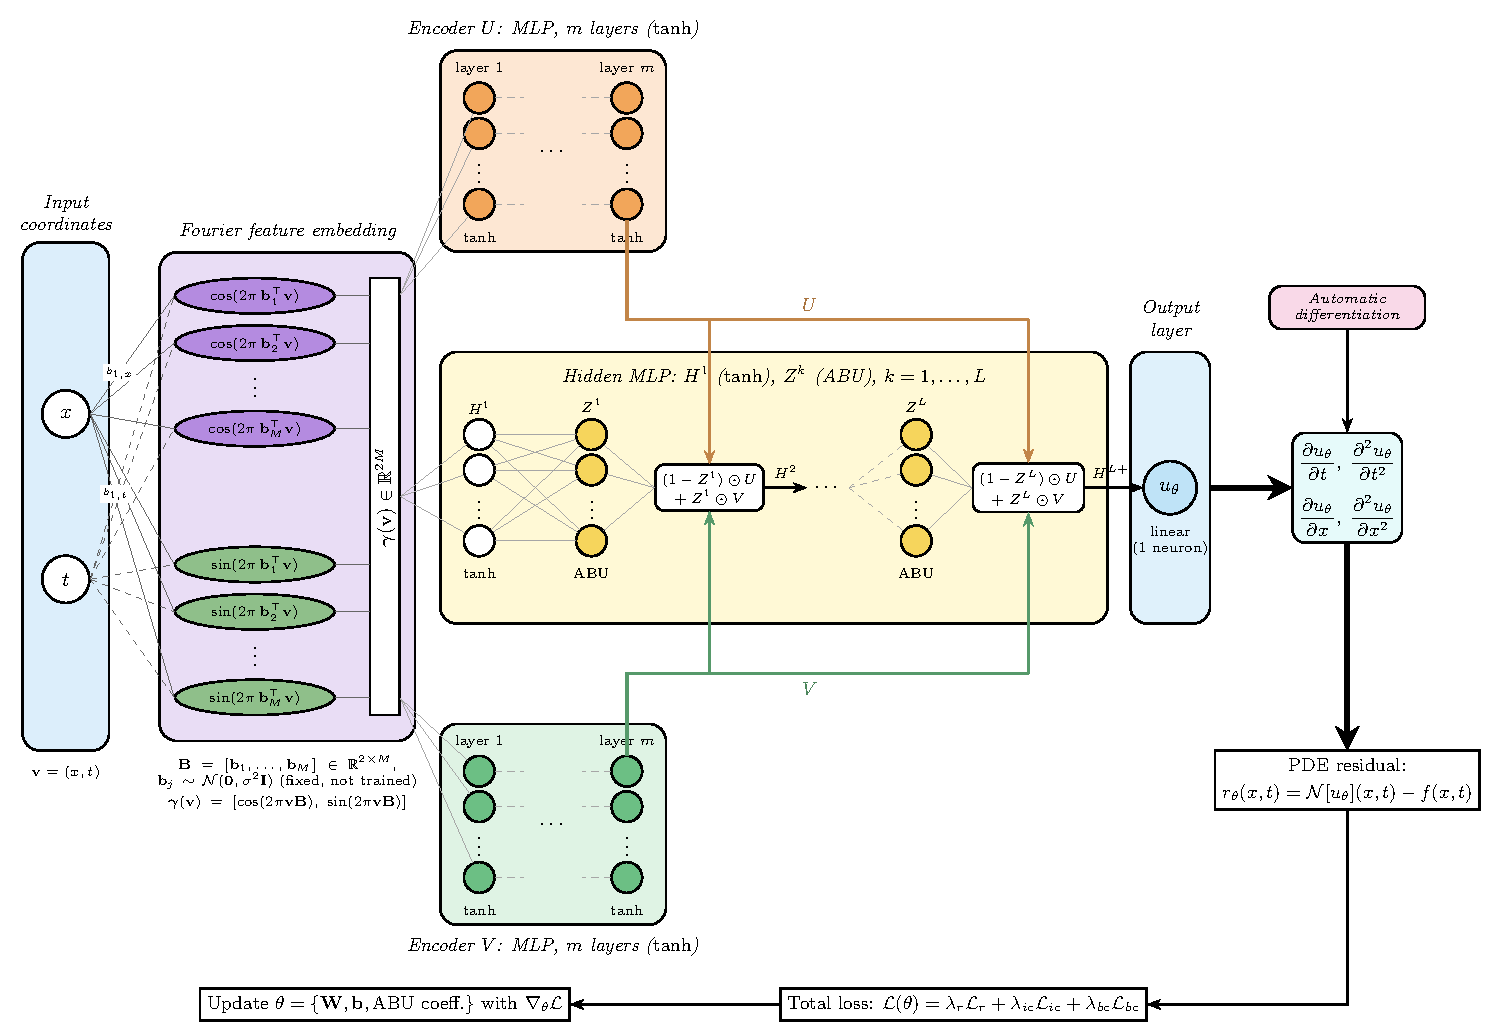
\includegraphics[width=\textwidth]{arquitectura_mABU.pdf}
% ============================================================
\documentclass[tikz,border=6pt]{standalone}
\usepackage{amsmath,amssymb,bm}
\usetikzlibrary{positioning,calc,fit,backgrounds,decorations.pathreplacing,arrows.meta,shapes.geometric}

% ---------- Colores (cámbialos a tu gusto) ----------
\definecolor{cIn}{HTML}{DCEEFB}
\definecolor{cFF}{HTML}{E9DDF5}   \definecolor{cFFcos}{HTML}{B48BE0} \definecolor{cFFsin}{HTML}{8FBF8A}
\definecolor{cU}{HTML}{FDE7D3}    \definecolor{cUn}{HTML}{F2A65A}
\definecolor{cV}{HTML}{DFF3E4}    \definecolor{cVn}{HTML}{6CBF84}
\definecolor{cH}{HTML}{FFF9D6}    \definecolor{cHt}{HTML}{FFFFFF}   \definecolor{cHa}{HTML}{F6D55C}
\definecolor{cOut}{HTML}{BFE3F7}  \definecolor{cAD}{HTML}{F9D9E8}  \definecolor{cRes}{HTML}{E6FAFA}

\tikzset{
  >={Stealth[length=2.2mm]},
  neuron/.style={circle,draw,thick,minimum size=5.2mm,inner sep=0pt},
  panel/.style={draw,rounded corners=8pt,thick,inner sep=7pt},
  ff/.style={ellipse,draw,thick,minimum height=6mm,minimum width=27mm,inner sep=1pt,font=\scriptsize},
  gate/.style={draw,thick,rounded corners=4pt,fill=white,font=\scriptsize,align=center,inner sep=3pt},
  conn/.style={gray!70,line width=0.3pt},
  dconn/.style={gray!70,line width=0.3pt,dashed},
  title/.style={font=\small\itshape,align=center},
  dims/.style={font=\scriptsize,align=center},
  bus/.style={very thick,->},
}

% Columna de neuronas: \ncol{nombre}{x}{y centro}{color}
% crea nombre-1, nombre-2, nombre-3 (arriba), puntos y nombre-4 (abajo)
\newcommand{\ncol}[4]{%
  \node[neuron,fill=#4] (#1-1) at (#2,#3+1.05) {};
  \node[neuron,fill=#4] (#1-2) at (#2,#3+0.45) {};
  \node at (#2,#3-0.12) {$\vdots$};
  \node[neuron,fill=#4] (#1-4) at (#2,#3-0.75) {};
}
% Conexión densa entre dos columnas
\newcommand{\dense}[3][conn]{%
  \foreach \i in {1,2,4}{\foreach \j in {1,2,4}{\draw[#1] (#2-\i) -- (#3-\j);}}}

\begin{document}
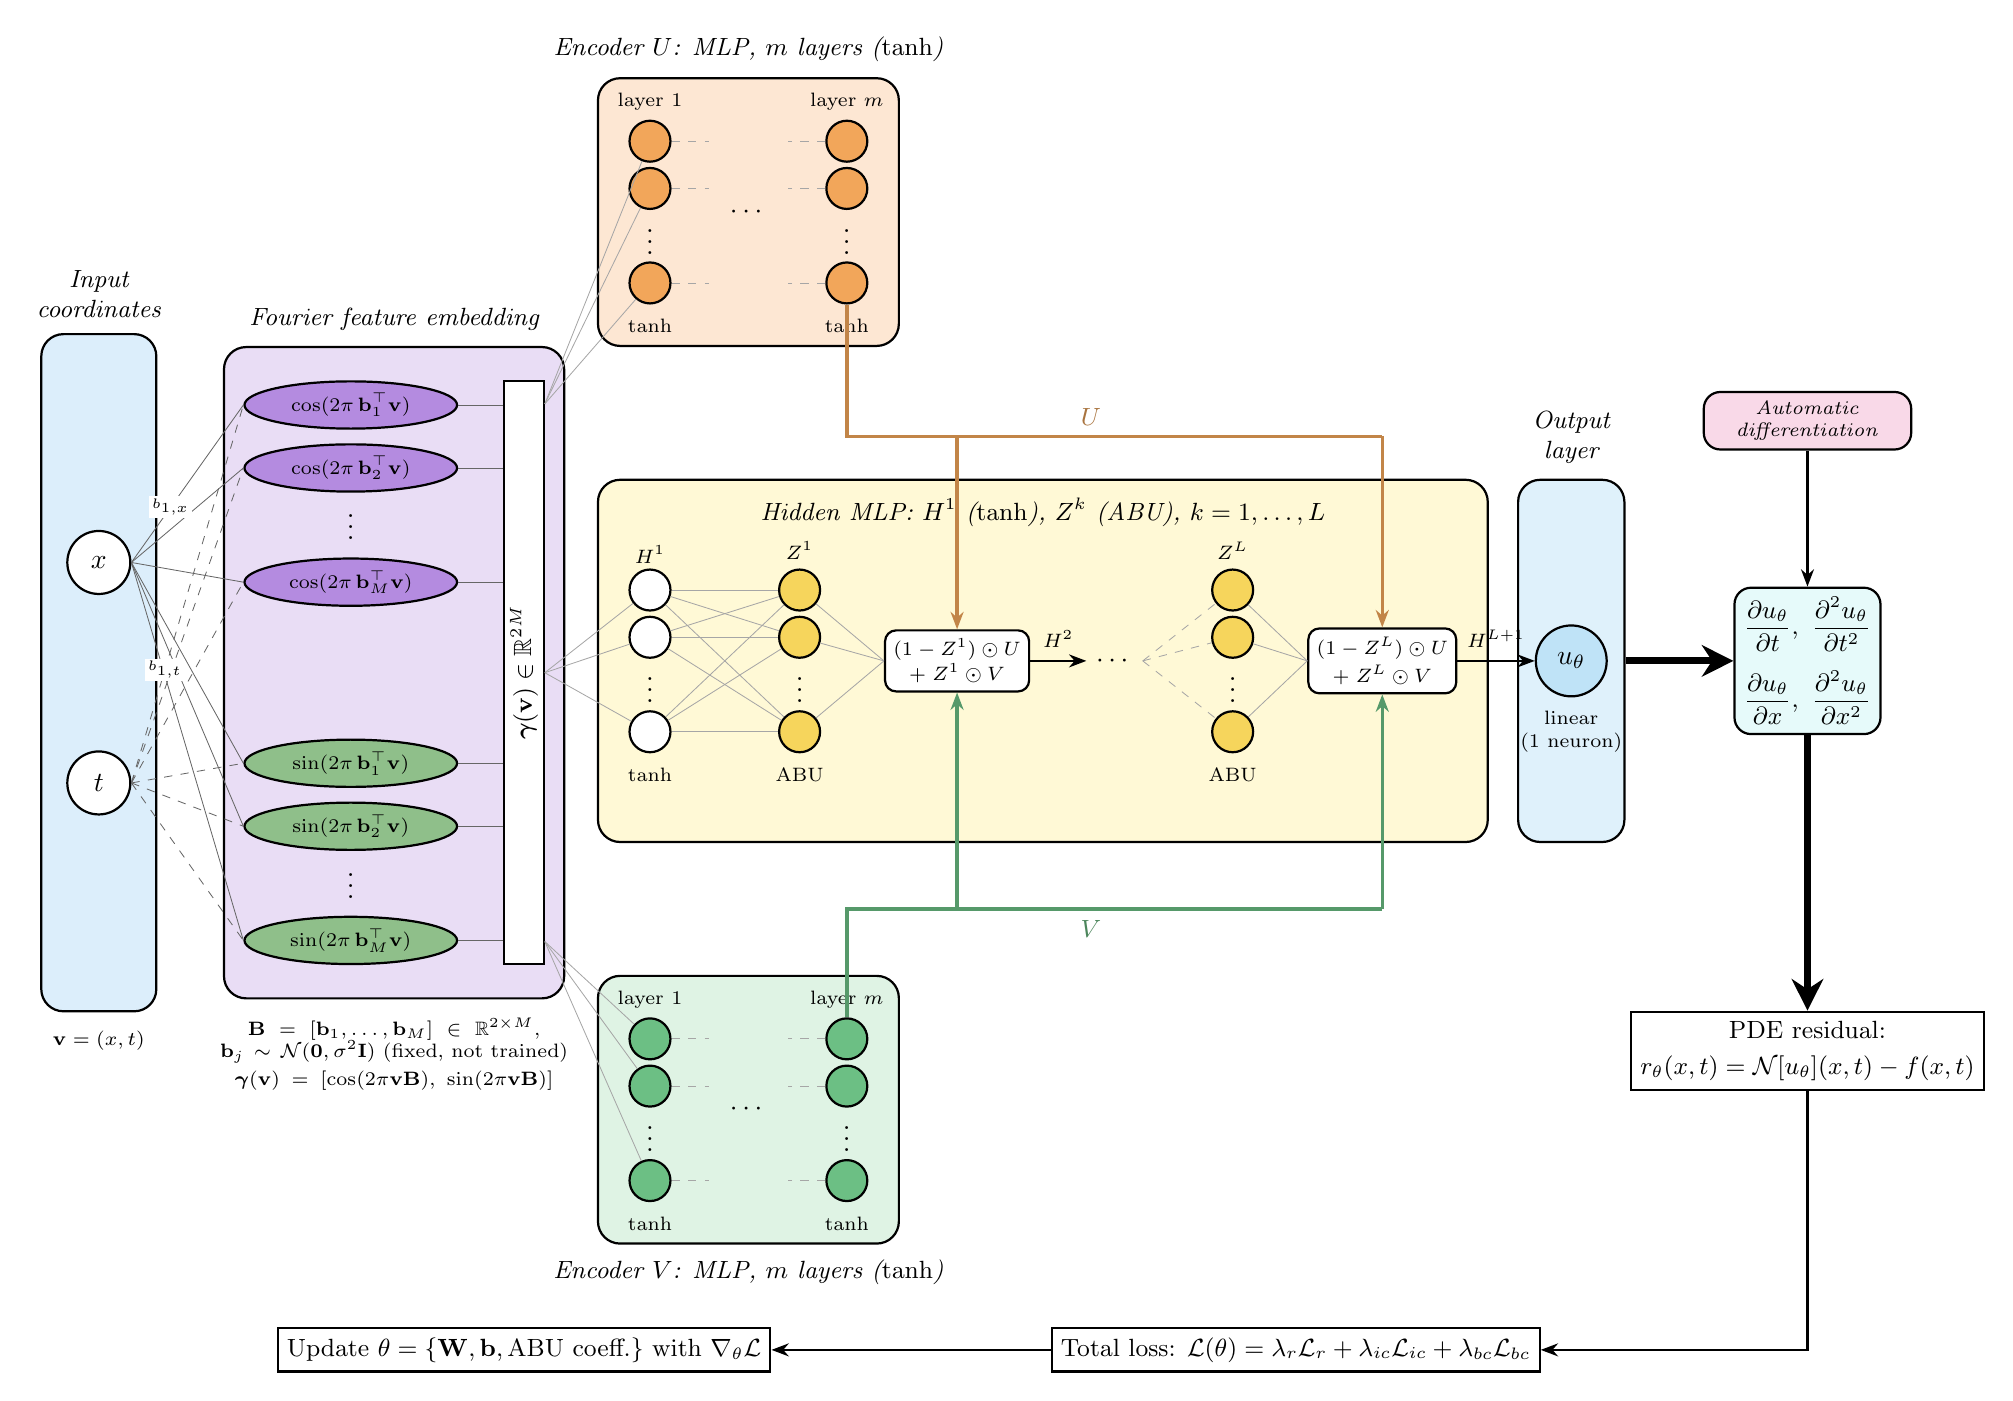
\begin{tikzpicture}

% ================= 1. Entradas =================
\node[neuron,minimum size=8mm,fill=white] (x) at (0, 1.4) {$x$};
\node[neuron,minimum size=8mm,fill=white] (t) at (0,-1.4) {$t$};

% ================= 2. Fourier embedding =================
\def\xf{3.2}
\node[ff,fill=cFFcos] (c1) at (\xf, 3.4) {$\cos(2\pi\,\mathbf b_1^{\top}\mathbf v)$};
\node[ff,fill=cFFcos] (c2) at (\xf, 2.6) {$\cos(2\pi\,\mathbf b_2^{\top}\mathbf v)$};
\node at (\xf,1.95) {$\vdots$};
\node[ff,fill=cFFcos] (cM) at (\xf, 1.15) {$\cos(2\pi\,\mathbf b_M^{\top}\mathbf v)$};
\node[ff,fill=cFFsin] (s1) at (\xf,-1.15) {$\sin(2\pi\,\mathbf b_1^{\top}\mathbf v)$};
\node[ff,fill=cFFsin] (s2) at (\xf,-1.95) {$\sin(2\pi\,\mathbf b_2^{\top}\mathbf v)$};
\node at (\xf,-2.6) {$\vdots$};
\node[ff,fill=cFFsin] (sM) at (\xf,-3.4) {$\sin(2\pi\,\mathbf b_M^{\top}\mathbf v)$};

% cada feature depende de x y de t (b_j = (b_{j,x}, b_{j,t}))
\foreach \n in {c1,c2,cM,s1,s2,sM}{
  \draw[conn,black!60] (x.east) -- (\n.west);
  \draw[conn,black!60,dashed] (t.east) -- (\n.west);
}
\node[font=\tiny,fill=white,inner sep=1pt] at ($(x.east)!0.35!(c1.west)$) {$b_{1,x}$};
\node[font=\tiny,fill=white,inner sep=1pt] at ($(t.east)!0.30!(c1.west)$) {$b_{1,t}$};

% vector embebido gamma(v)
\node[draw,thick,fill=white,minimum width=5mm,minimum height=74mm,inner sep=0pt] (gam) at (5.4,0) {};
\node[rotate=90,font=\small] at (gam) {$\bm\gamma(\mathbf v)\in\mathbb R^{2M}$};
\foreach \n in {c1,c2,cM,s1,s2,sM}{\draw[conn,black!60] (\n.east) -- (gam.west |- \n);}

% ================= 3. Encoder U (arriba) =================
\def\yU{5.7}
\ncol{U1}{7.0}{\yU}{cUn}
\node (Udots) at (8.25,\yU+0.15) {$\cdots$};
\ncol{Um}{9.5}{\yU}{cUn}
\foreach \i in {1,2,4}{\draw[dconn] (U1-\i) -- ++(0.75,0); \draw[dconn] (Um-\i) -- ++(-0.75,0);}
\foreach \j in {1,2,4}{\draw[conn] ($(gam.north east)+(0,-0.3)$) -- (U1-\j);}
\node[dims] at (7.0,\yU-1.3) {$\tanh$}; \node[dims] at (9.5,\yU-1.3) {$\tanh$};
\node[dims] at (7.0,\yU+1.55) {layer $1$}; \node[dims] at (9.5,\yU+1.55) {layer $m$};

% ================= 4. Encoder V (abajo) =================
\def\yV{-5.7}
\ncol{V1}{7.0}{\yV}{cVn}
\node (Vdots) at (8.25,\yV+0.15) {$\cdots$};
\ncol{Vm}{9.5}{\yV}{cVn}
\foreach \i in {1,2,4}{\draw[dconn] (V1-\i) -- ++(0.75,0); \draw[dconn] (Vm-\i) -- ++(-0.75,0);}
\foreach \j in {1,2,4}{\draw[conn] ($(gam.south east)+(0,0.3)$) -- (V1-\j);}
\node[dims] at (7.0,\yV-1.3) {$\tanh$}; \node[dims] at (9.5,\yV-1.3) {$\tanh$};
\node[dims] at (7.0,\yV+1.55) {layer $1$}; \node[dims] at (9.5,\yV+1.55) {layer $m$};

% ================= 5. Hidden MLP (centro) =================
\ncol{H1}{7.0}{0}{cHt}
\foreach \j in {1,2,4}{\draw[conn] (gam.east) -- (H1-\j);}
\ncol{Z1}{8.9}{0}{cHa}
\dense{H1}{Z1}
\node[gate] (g1) at (10.9,0.15) {$(1-Z^{1})\odot U$\\[1pt]$+\;Z^{1}\odot V$};
\foreach \i in {1,2,4}{\draw[conn] (Z1-\i) -- (g1.west);}
\node (Hdots) at (12.9,0.15) {$\cdots$};
\draw[->,thick] (g1.east) -- node[above=1pt,font=\scriptsize]{$H^{2}$} (Hdots.west);
\ncol{ZL}{14.4}{0}{cHa}
\foreach \j in {1,2,4}{\draw[dconn] (Hdots.east) -- (ZL-\j);}
\node[gate] (gL) at (16.3,0.15) {$(1-Z^{L})\odot U$\\[1pt]$+\;Z^{L}\odot V$};
\foreach \i in {1,2,4}{\draw[conn] (ZL-\i) -- (gL.west);}

\node[dims] at (7.0,-1.3) {$\tanh$};
\node[dims] at (8.9,-1.3) {ABU};
\node[dims] at (14.4,-1.3) {ABU};
\node[dims] at (7.0,1.5) {$H^{1}$};
\node[dims] at (8.9,1.55) {$Z^{1}$};
\node[dims] at (14.4,1.55) {$Z^{L}$};

% Buses U y V hacia todas las compuertas
\coordinate (Ubus) at (10.2,3.0);
\coordinate (Vbus) at (10.2,-3.0);
\draw[very thick,cUn!80!black] (Um-4.south) |- ($(Ubus)$) -- (gL.north |- Ubus);
\draw[very thick,cVn!80!black] (Vm-1.north) |- ($(Vbus)$) -- (gL.south |- Vbus);
\node[font=\small,text=cUn!70!black] at (12.6,3.25) {$U$};
\node[font=\small,text=cVn!70!black] at (12.6,-3.25) {$V$};
\foreach \g in {g1,gL}{
  \draw[->,very thick,cUn!80!black] (\g.north |- Ubus) -- (\g.north);
  \draw[->,very thick,cVn!80!black] (\g.south |- Vbus) -- (\g.south);
}

% ================= 6. Salida =================
\node[neuron,minimum size=9mm,fill=cOut,thick] (u) at (18.7,0.15) {$u_\theta$};
\draw[->,thick] (gL.east) -- node[above=1pt,font=\scriptsize]{$H^{L+1}$} (u.west);
\node[dims] at (18.7,-0.75) {linear\\(1 neuron)};

% ================= Paneles de fondo =================
\begin{scope}[on background layer]
  \node[panel,fill=cIn,fit=(x)(t),minimum height=86mm,inner xsep=9pt] (Pin) {};
  \node[panel,fill=cFF,fit=(c1)(sM)(gam),inner ysep=12pt] (Pff) {};
  \node[panel,fill=cU,fit=(U1-1)(Um-4)(Udots),inner sep=11pt,yshift=0pt,minimum height=34mm] (PU) {};
  \node[panel,fill=cV,fit=(V1-1)(Vm-4)(Vdots),inner sep=11pt,minimum height=34mm] (PV) {};
  \node[panel,fill=cH,fit=(H1-1)(H1-4)(gL)(g1),inner sep=11pt,minimum height=46mm] (PH) {};
  \node[panel,fill=cOut!50,fit=(u),minimum height=46mm,inner xsep=6pt] (Pout) {};
\end{scope}

% ================= Títulos =================
\node[title,above=2pt of Pin.north] {Input\\coordinates};
\node[title,above=2pt of Pff.north] {Fourier feature embedding};
\node[title,above=2pt of PU.north] {Encoder $U$: MLP, $m$ layers ($\tanh$)};
\node[title,below=2pt of PV.south] {Encoder $V$: MLP, $m$ layers ($\tanh$)};
\node[title,anchor=north] at ($(PH.north)+(0,-0.12)$) {Hidden MLP: $H^{1}$ ($\tanh$), $Z^{k}$ (ABU), $k=1,\dots,L$};
\node[title,above=2pt of Pout.north] {Output\\layer};

\node[dims,below=3pt of Pin.south] {$\mathbf v=(x,t)$};
\node[dims,below=3pt of Pff.south,text width=50mm,align=center] {$\mathbf B=[\mathbf b_1,\dots,\mathbf b_M]\in\mathbb R^{2\times M}$,\\
  $\mathbf b_j\sim\mathcal N(\mathbf 0,\sigma^2\mathbf I)$ (fixed, not trained)\\[2pt]
  $\bm\gamma(\mathbf v)=[\cos(2\pi\mathbf v\mathbf B),\ \sin(2\pi\mathbf v\mathbf B)]$};

% ================= 7. Física: AD, residuo, pérdida =================
\node[draw,thick,rounded corners=6pt,fill=cAD,align=center,font=\scriptsize,text width=24mm] (ad) at (21.7,3.2)
  {\textit{Automatic}\\\textit{differentiation}};
\node[draw,thick,rounded corners=6pt,fill=cRes,align=center,font=\small] (der) at (21.7,0.15)
  {$\dfrac{\partial u_\theta}{\partial t},\ \dfrac{\partial^2 u_\theta}{\partial t^2}$\\[6pt]
   $\dfrac{\partial u_\theta}{\partial x},\ \dfrac{\partial^2 u_\theta}{\partial x^2}$};
\draw[-{Stealth[length=4mm,width=4mm]},line width=2.5pt] (Pout.east) -- (der.west);
\draw[->,thick] (ad) -- (der);

\node[draw,thick,fill=white,font=\small,align=center] (res) at (21.7,-4.8)
  {PDE residual:\\[2pt] $r_\theta(x,t)=\mathcal N[u_\theta](x,t)-f(x,t)$};
\draw[-{Stealth[length=4mm,width=4mm]},line width=2.5pt] (der.south) -- (res.north);

\node[draw,thick,fill=white,font=\small] (loss) at (15.2,-8.6)
  {Total loss: $\mathcal L(\theta)=\lambda_{r}\mathcal L_{r}+\lambda_{ic}\mathcal L_{ic}+\lambda_{bc}\mathcal L_{bc}$};
\draw[->,thick] (res.south) |- (loss.east);
\node[draw,thick,fill=white,font=\small] (upd) at (5.4,-8.6)
  {Update $\theta=\{\mathbf W,\mathbf b,\text{ABU coeff.}\}$ with $\nabla_\theta\mathcal L$};
\draw[->,thick] (loss.west) -- (upd.east);

\end{tikzpicture}
\end{document}
